\documentclass[12pt,compress,english,utf8,t]{beamer}

\usepackage{etex}

\usepackage[english]{babel}

\usepackage{ragged2e}
\usepackage{mathtools}
\usepackage[cmtip,all]{xy}
\newcommand{\longsquiggly}{\xymatrix{{}\ar@{~>}[r]&{}}}

\usepackage[protrusion=true,expansion=true]{microtype}

\title{Das Geheimnis der Zahl 5}
\author{Ingo Blechschmidt}
\institute{Tübinger Linuxtag}
\date{11. Juni 2016}

\usetheme{Warsaw}
\usecolortheme{seahorse}
\definecolor{mypurple}{RGB}{150,0,255}
\setbeamercolor{structure}{fg=mypurple}
\usefonttheme{serif}
\usepackage[T1]{fontenc}
\usepackage{libertine}
\useinnertheme{rectangles}
\setbeamercovered{invisible}

\setbeamertemplate{title page}[default][colsep=-1bp,rounded=false,shadow=false]
\setbeamertemplate{frametitle}[default][colsep=-2bp,rounded=false,shadow=false,center]

\setbeamertemplate{navigation symbols}{}
\setbeamertemplate{headline}{}

\newcommand*\oldmacro{}%
\let\oldmacro\insertshorttitle%
\renewcommand*\insertshorttitle{%
  \oldmacro\hfill\insertframenumber\,/\,\inserttotalframenumber\hfill}

\newcommand{\backupstart}{
  \newcounter{framenumberpreappendix}
  \setcounter{framenumberpreappendix}{\value{framenumber}}
}
\newcommand{\backupend}{
  \addtocounter{framenumberpreappendix}{-\value{framenumber}}
  \addtocounter{framenumber}{\value{framenumberpreappendix}} 
}

\newcommand{\defeq}{\vcentcolon=}

\newcommand{\hil}[1]{{\usebeamercolor[fg]{item}{\textbf{#1}}}}

\newcommand{\icfrac}[4]{#1 + \dfrac{1}{#2 + \dfrac{1}{#3 + \dfrac{1}{#4 + \ddots}}}}
\newcommand{\icfracc}[3]{\dfrac{1}{#1 + \dfrac{1}{#2 + \dfrac{1}{#3 + \ddots}}}}
\newcommand{\icfraccc}[2]{\dfrac{1}{#1 + \dfrac{1}{#2 + \ddots}}}
\newcommand{\icfracccc}[5]{#1 + \dfrac{1}{#2 + \dfrac{1}{#3 + \dfrac{1}{#4 + \dfrac{1}{#5 + \ddots}}}}}

\setbeameroption{show notes}
\setbeamertemplate{note page}[plain]

\begin{document}

\frame{
  \titlepage

  \vspace*{-2em}
  \begin{center}
    \small
    \emph{Gewidmet an Prof. Dr. Jost-Hinrich Eschenburg.}
    \medskip

    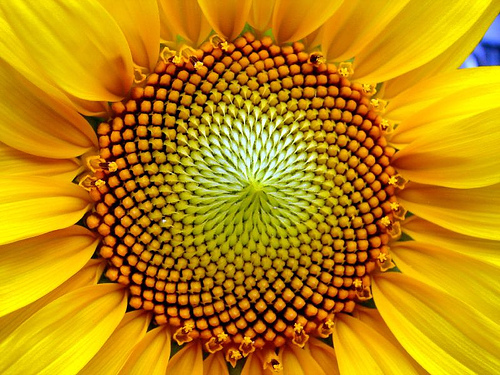
\includegraphics[height=0.25\textheight]{sonnenblume}\quad
    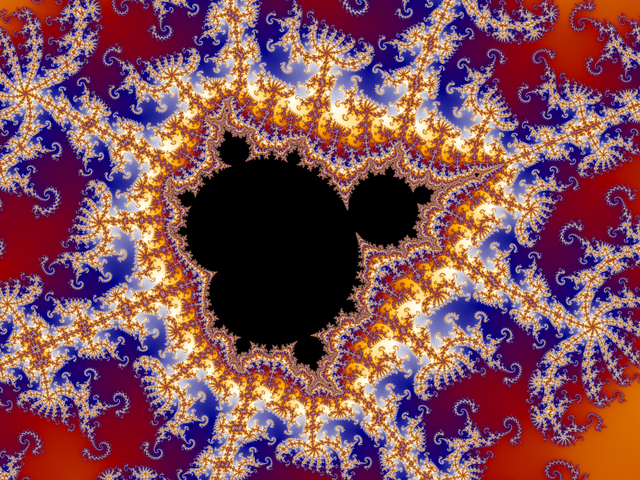
\includegraphics[height=0.25\textheight]{mandelbrot}\quad
    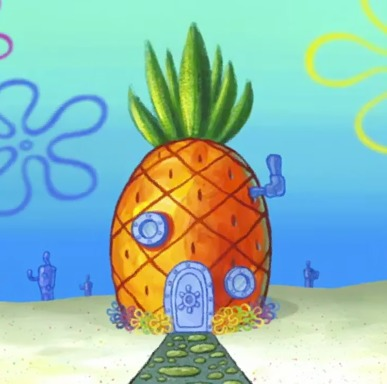
\includegraphics[height=0.25\textheight]{spongebob-ananas}
  \end{center}
}

\begin{frame}\frametitle{Gliederung}\tableofcontents\end{frame}


\section{Ein Entwurfsmuster der Natur}

\begin{frame}\frametitle{Ein Entwurfsmuster der Natur}
  \begin{center}
    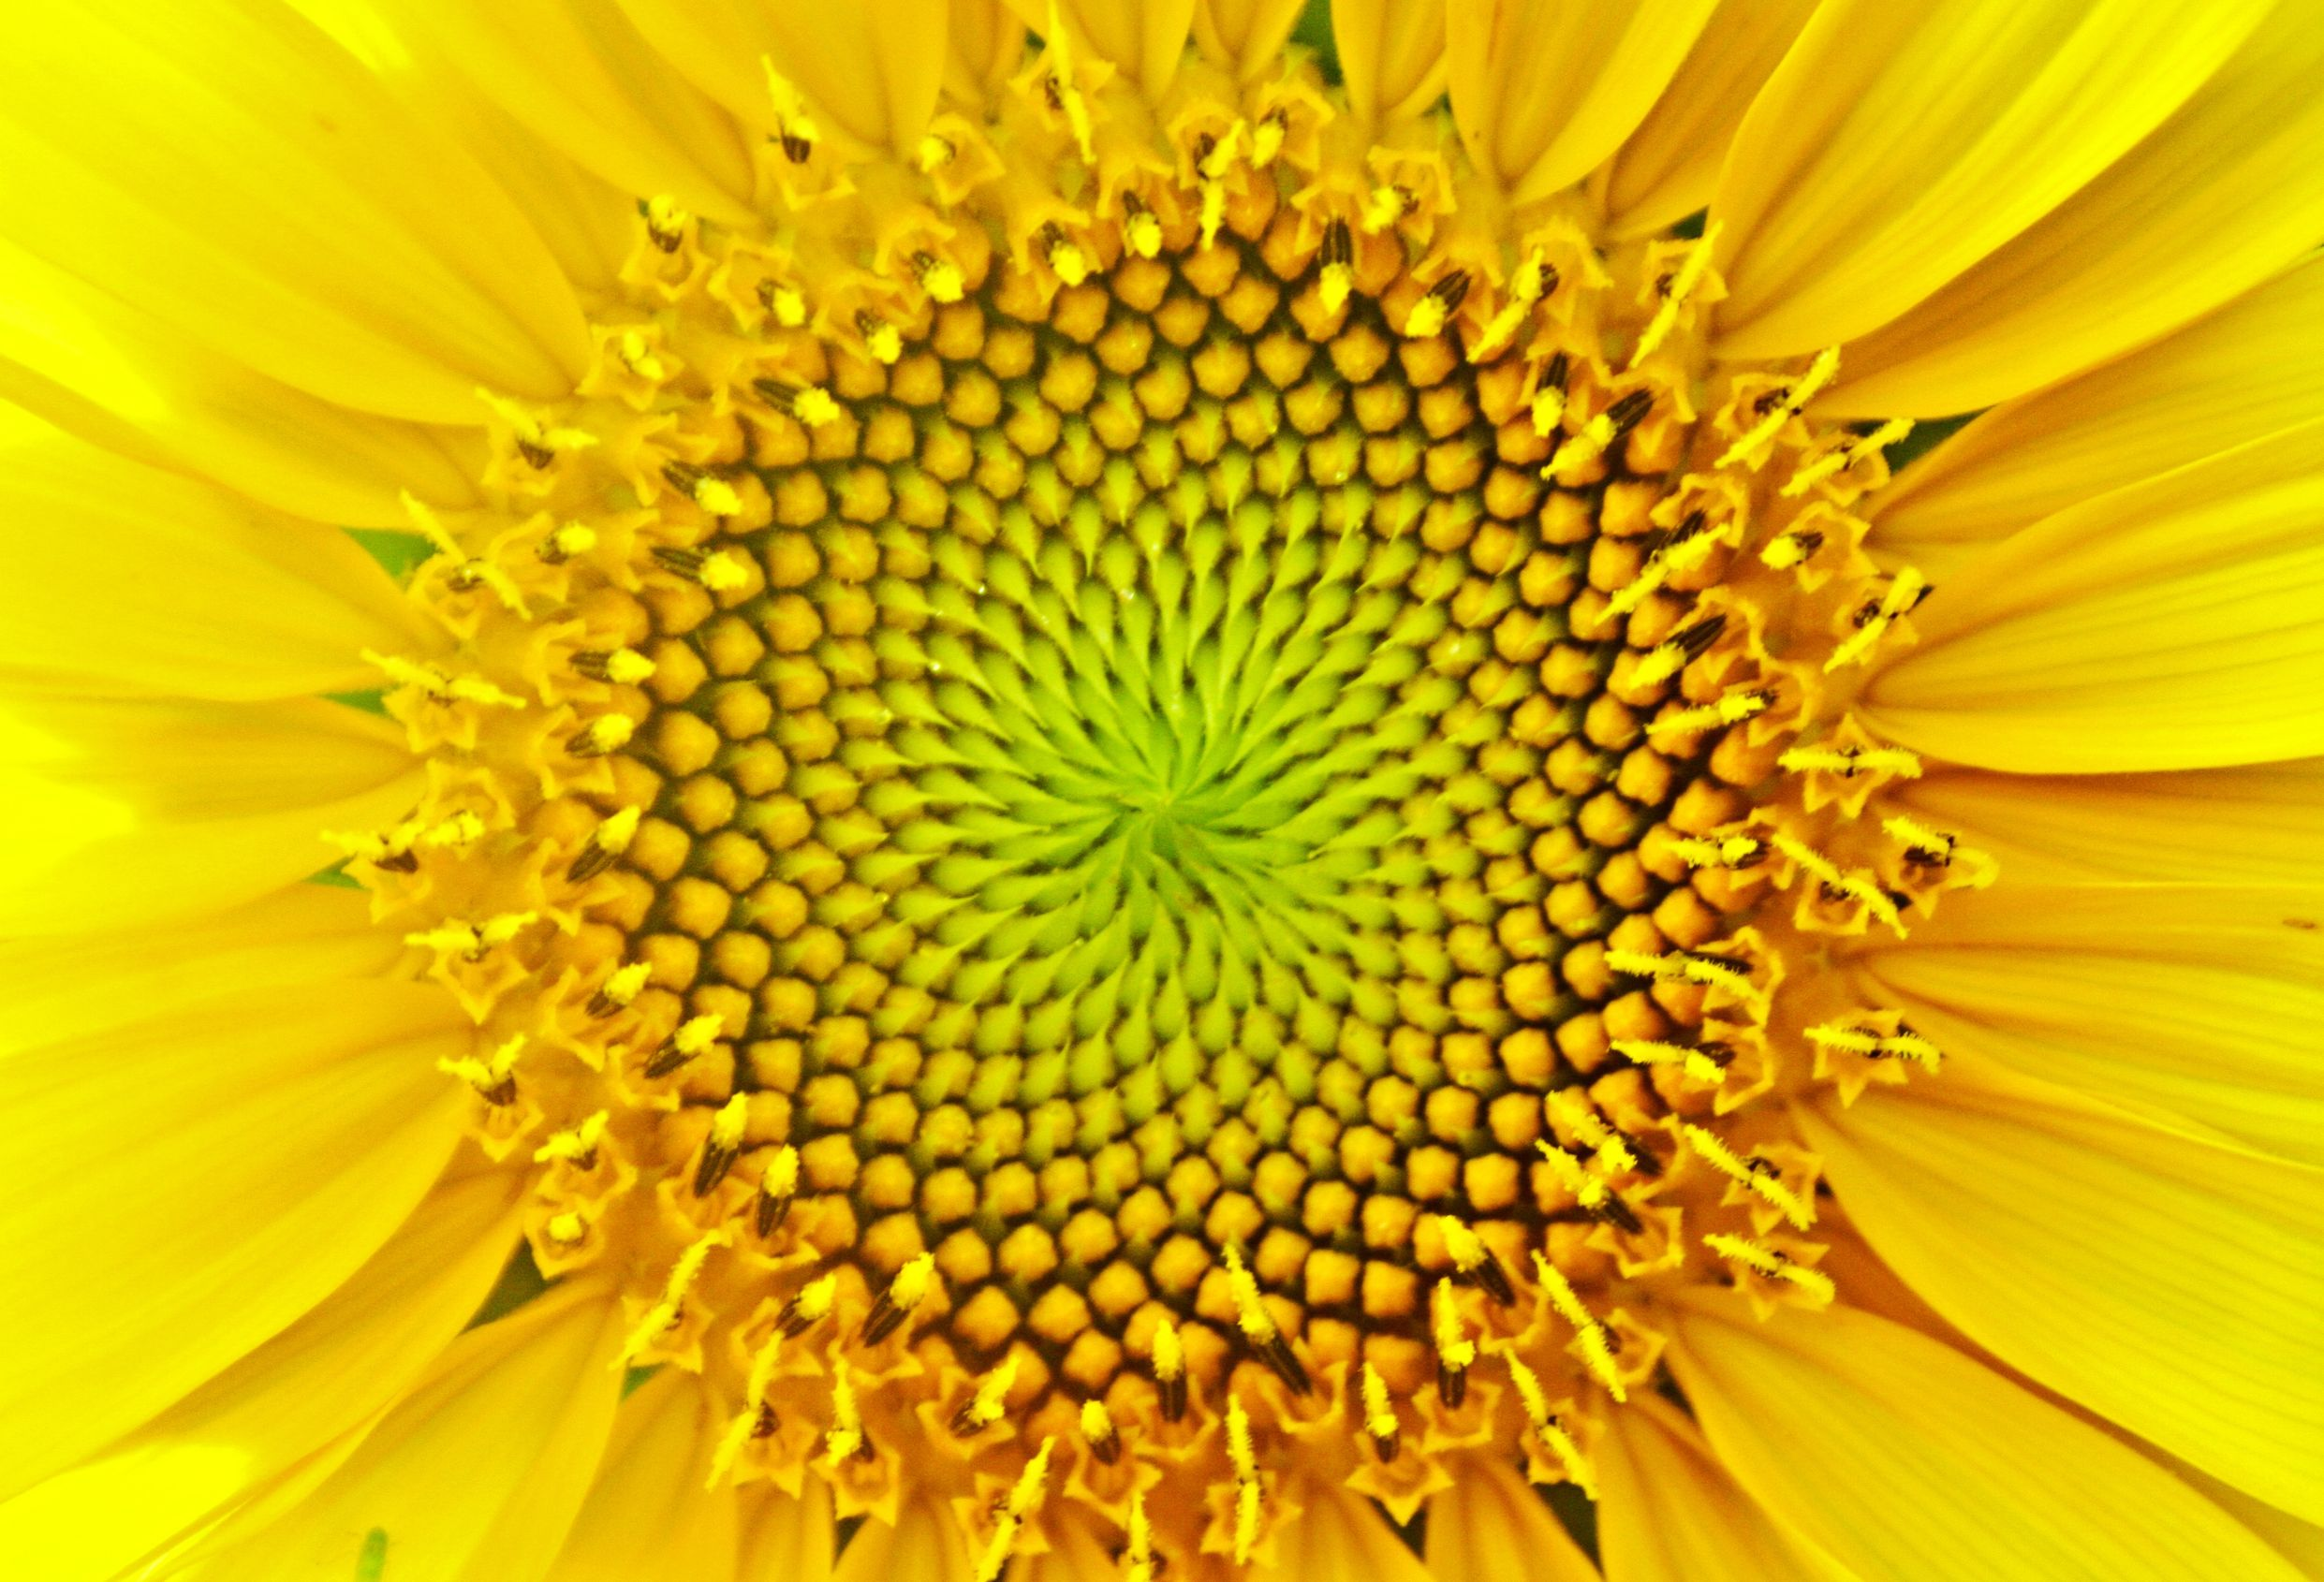
\includegraphics[height=0.6\textheight]{sonnenblume2}
    \bigskip
    % 34 counterclockwise, 21 clockwise

    \only<1>{
      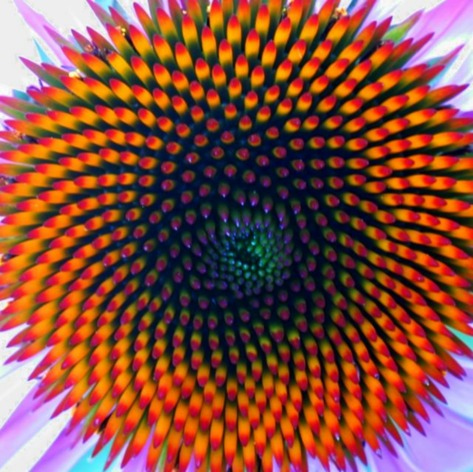
\includegraphics[height=0.2\textheight]{coneflower}\qquad
      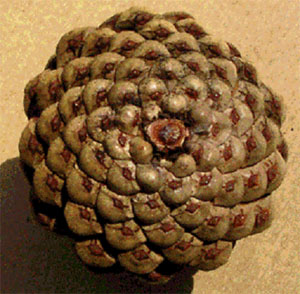
\includegraphics[height=0.2\textheight]{zapfen}\qquad
      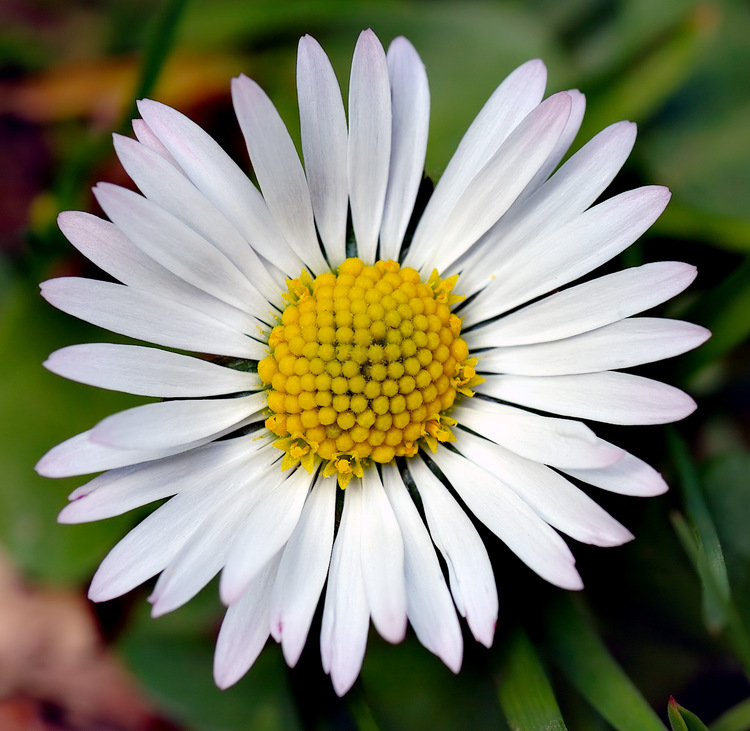
\includegraphics[height=0.2\textheight]{Bellis_perennis_white_(aka)}
    }
    \only<2>{
      \hil{Fibonaccizahlen:} \\
      1, 1, 2, 3, 5, 8, 13, 21, 34, 55, \ldots
    }
  \end{center}
\end{frame}

\note{\justifying
  The number of spirals on a sunflower is always a Fibonacci number (or a
  number very close to a Fibonacci number), for instance in the large picture
  on the previous slide there are 21 clockwise spirals and 34
  counterclockwise ones. Why?
  \par
}


\section{Kettenbrüche}

\subsection{Beispiele}

\begin{frame}\frametitle{Ein merkwürdiger Bruch}
  \only<2-3>{\vspace*{-1em}}
  \only<1>{\Huge}
  \only<1-3>{\[
    \icfrac{1}{2}{2}{2} = {?}
  \]}
  \only<2-3>{\vspace*{1em}}

  \pause
  Entscheidende Beobachtung: Wenn wir
  \only<1-3>{\[ x \defeq {?} - 1 = \icfracc{2}{2}{2}, \]}
  \only<4->{\[ x \defeq {?} - 1 = \icfraccc{2}{2}, \]}
  \pause
  setzen, gilt
  \[ \frac{1}{2 + x} = x. \]
  \pause
  \pause

  Multiplizieren mit dem Nenner liefert
  \only<5>{$1 = x \cdot (2 + x),$}%
  \only<6->{$1 = 2x + x^2,$}
  \pause
  \pause
  also müssen wir nur die quadratische Gleichung
  $0 = x^2 + 2x - 1$
  lösen,
  \pause
  somit
  \[ x = \frac{-2 + \sqrt{8}}{2} = -1 + \sqrt{2}
    \quad\text{oder}\quad
     x = \frac{-2 - \sqrt{8}}{2} = -1 - \sqrt{2}. \]
  Es ist die positive Möglichkeit.
\end{frame}

\begin{frame}\frametitle{Weitere Beispiele}
  \only<1-2>{\vspace*{-2em}\begin{align*}
    \visible<2>{[1; 2, 2, 2, \ldots] =} \icfrac{1}{2}{2}{2} &= \sqrt{2} \\[1.5em]
    \visible<2>{[2; 4, 4, 4, \ldots] =} \icfrac{2}{4}{4}{4} &= \sqrt{5} \\[1.5em]
    \visible<2>{[3; 6, 6, 6, \ldots] =} \icfrac{3}{6}{6}{6} &= \sqrt{10}
  \end{align*}}

  \pause
  \pause

  \begin{enumerate}
    \item $\phantom{0}\sqrt{2} = [1; 2, 2, 2, 2, 2, 2, 2, 2, \ldots]$
    \item $\phantom{0}\sqrt{5} = [2; 4, 4, 4, 4, 4, 4, 4, 4, \ldots]$
    \item $\sqrt{10}           = [3; 6, 6, 6, 6, 6, 6, 6, 6, \ldots]$
    \item $\phantom{0}\sqrt{6} = [2; 2, 4, 2, 4, 2, 4, 2, 4, \ldots]$
    \item $\sqrt{14}           = [3; 1, 2, 1, 6, 1, 2, 1, 6, \ldots]$
    \item $\sbox0{$\sqrt{10}$}\makebox[\wd0][l]{$e$} = [2; 1, 2, 1, 1, 4, 1, 1, 6, \ldots]$
  \end{enumerate}
\end{frame}

\note{\justifying
  The digits of the number~$e = 2.7182818284\ldots$, the basis of the natural
  logarithm, do not have any concernible pattern. But its continued fraction
  expansion is completely regular.\par
}


\subsection{Berechnung der Kettenbruchentwicklung}

\begin{frame}\frametitle{Der euklidische Algorithmus}
  Zur Erinnerung: $\sqrt{2} = [1; 2, 2, 2, \ldots] = 1.41421356\ldots$
  \begin{align*}
    1.41421356\ldots &= 1 \cdot 1.00000000\ldots + 0.41421356\ldots \\
    1.00000000\ldots &= 2 \cdot 0.41421356\ldots + 0.17157287\ldots \\
    0.41421356\ldots &= 2 \cdot 0.17157287\ldots + 0.07106781\ldots \\
    0.17157287\ldots &= 2 \cdot 0.07106781\ldots + 0.02943725\ldots \\
    0.07106781\ldots &= 2 \cdot 0.02943725\ldots + 0.01219330\ldots \\
    0.02943725\ldots &= 2 \cdot 0.01219330\ldots + 0.00505063\ldots \\
    &\,\,\,\vdots
  \end{align*}
\end{frame}

\note{\justifying
  Why does the Euclidean algorithm give the continued fraction coefficients?
  Let's write
  \begin{align*}
    x   &= a_0 \cdot \sbox0{$r_0$}\makebox[\wd0][l]{$1$} + r_0 \\
    1   &= a_1 \cdot r_0 + r_1 \\
    r_0 &= a_2 \cdot r_1 + r_2 \\
    r_1 &= a_3 \cdot r_2 + r_3
  \end{align*}
  and so on, where the numbers~$a_n$ are natural numbers and the residues~$r_n$
  are smaller than the second factor of the respective adjacent product. Then:
  \begin{align*}
    x &= a_0 + r_0 = a_0 + 1/(1/r_0) \\
      &= a_0 + 1/(a_1 + r_1/r_0) = a_0 + 1/(a_1 + 1/(r_0/r_1)) \\
      &= a_0 + 1/(a_1 + 1/(a_2 + r_2/r_1)) = \cdots
  \end{align*}
}

\note{\justifying
  In the beautiful language Haskell, the code for lazily calculating the
  infinite continued fraction expansion is only one line long (the type
  declaration is optional).
  \medskip

  {\scriptsize\texttt{cf :: Double -> [Integer]}\\
  \texttt{cf x = a : cf (1 / (x - fromIntegral a)) where a = floor x}\par}
  \medskip

  So the continued fraction expansion of a number~$x$ begins
  with~$a$, the integral part of~$x$, and continues with the
  continued fraction expansion of~$1 / (x-a)$.
  \medskip

  Note that because of floating-point inaccuracies, only the first few terms of
  the expansion are reliable. For instance,~\texttt{cf (sqrt 6)} could yield
  \[ \scriptsize\texttt{[2,2,4,2,4,2,4,2,4,2,4,2,4,2,4,2,2,1,48,2,4,6,1,\ldots\!\!]}. \]
  \par
}


\subsection{Bestapproximationen durch die Kettenbruchentwicklung}

\begin{frame}\frametitle{Bestapproximationen durch Kettenbrüche}
  \begin{theorem}
  Wenn man die Kettenbruchentwicklung einer Zahl~$x$ abschneidet, erhält man
  einen Bruch~$a/b$, der unter allen Brüchen mit Nenner~$\leq b$ der Zahl~$x$
  am nächsten liegt.
  \end{theorem}
  \[
    \sqrt{2} = \icfrac{1}{2}{2}{2} \longsquiggly
    1 + \dfrac{1}{2 + \dfrac{1}{2 + \dfrac{1}{2}}} = \frac{17}{12} \approx 1.42
  \]
  \medskip
  \pause

  \hil{Bonus.} Je größer der Koeffizient nach der Abschneidestelle ist, desto
  besser ist die Näherung~$a/b$.
\end{frame}

\note{\justifying
  More precisely, the bonus statement is that the distance from~$x$ to~$a/b$ is
  less than~$1 / (a_n a_{n+1})$, where~$a_n$ is the last coefficient to be
  included in the cut-off and~$a_{n+1}$ is the first coefficient after the
  cut-off.
  \par
}


\section{\texorpdfstring{Approximationen von $\pi$}{Approximationen von π}}

\begin{frame}[plain,c]
  \centering\Huge
  \scalebox{2.8}{\hil{Liebe ist}} \\[0.6em]
  \scalebox{2.8}{\hil{wichtig.}}

  \bigskip
  \bigskip

  \scalebox{2.8}{\hil{$\boldsymbol{\heartsuit}$}}
  \par
\end{frame}

\begin{frame}[plain,c]
  \centering\Huge
  \scalebox{2.8}{\hil{Pi ist}} \\[0.6em]
  \scalebox{2.8}{\hil{wichtig.}}

  \bigskip
  \bigskip

  \scalebox{2.8}{\hil{$\boldsymbol{\pi}$}}
  \par
\end{frame}

\begin{frame}\frametitle{Approximationen von $\pi$}
  \[ \pi = 3.1415926535\ldots = \icfracccc{3}{7}{15}{1}{292} \]

  \begin{enumerate}
    \item $3$
    \item $[3;7]\phantom{,15,1} = \phantom{0}22/7\phantom{00} = \underline{3.14}28571428\ldots$
    \item $[3;7,15]\phantom{,1} = 333/106 = \underline{3.1415}094339\ldots$
    \item $[3;7,15,1] = 355/113 = \underline{3.141592}9203\ldots$ (Milü)
  \end{enumerate}
\end{frame}

\note{\justifying
  We do not know for sure how people in ancient times calculated approximations
  to~$\pi$. But one possibility is that they used some form of the Euclidean
  algorithm (of course not using decimal expansions, but for instance strings
  of various lengths).
  \medskip

  Because the coefficient~$292$ appearing in the continued fraction expansion
  of~$\pi$ is exceptionally large, the approximation~$355/113$ is exceptionally
  good. That's a nice mathematical accident! I like to think that better
  approximations were not physically obtainable in ancient times, but thanks to
  this accident the best approximation that was obtainable was in fact an
  extremely good one. In particular, it's much better than the
  denominator~$113$ might want us to think.
  \medskip

  NB: The fraction~$355/113$ is easily memorized (11--33--55).
  \par
}


\section{Das Mandelbrot-Fraktal}

\begin{frame}\frametitle{Das Mandelbrot-Fraktal}
  \centering
  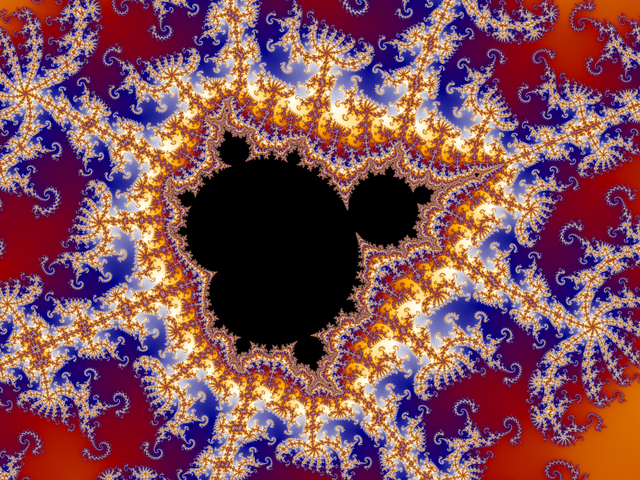
\includegraphics[width=0.8\textwidth]{mandelbrot}
  \medskip
  \pause

  Im Mandelbrot-Fraktal tauchen die Fibonaccizahlen auf.
  \par
\end{frame}

\note{\justifying
  See \url{http://math.bu.edu/DYSYS/FRACGEOM2/node7.html} for an explanation of
  where and why the Fibonacci numbers show up in the Mandelbrot fractal.\par
}


\section{Spiralen in der Natur}

\begin{frame}\frametitle{Spiralen in der Natur}
  \centering
  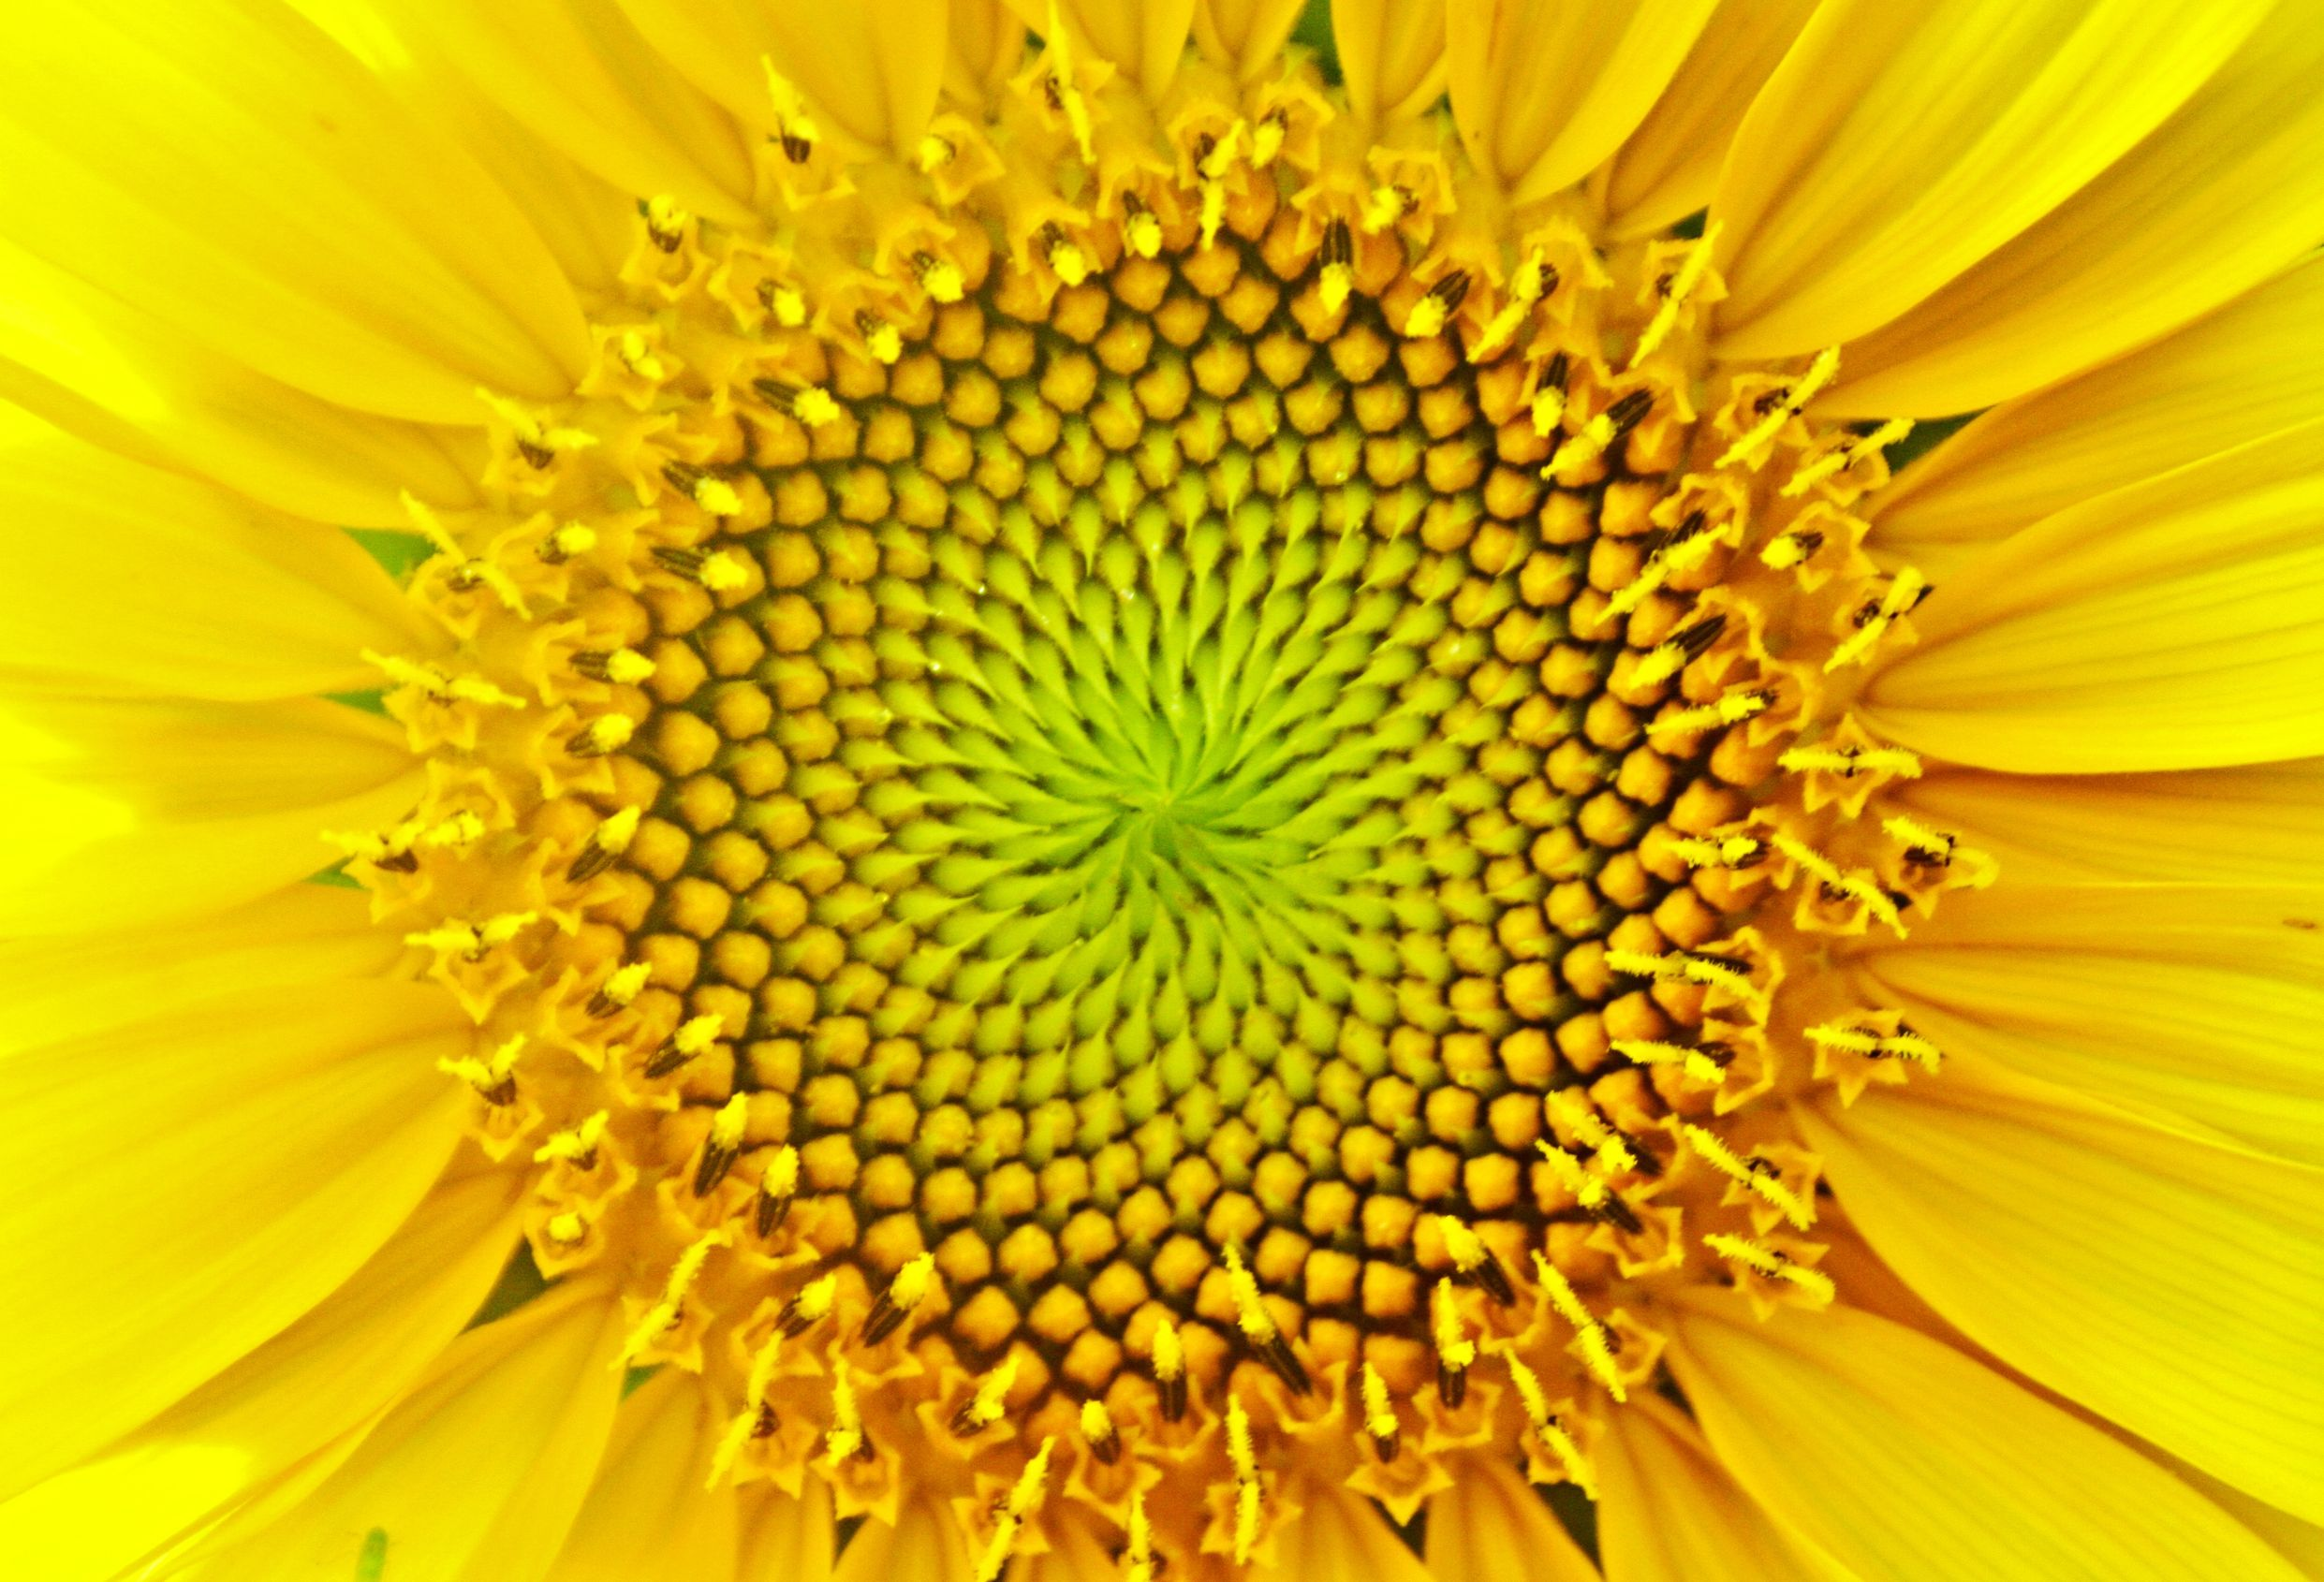
\includegraphics[height=0.8\textheight]{sonnenblume2}
  \par
\end{frame}

\begin{frame}\frametitle{Die irrationalste aller Zahlen}
  Für Pflanzen ist der optimale Winkel für aufeinanderfolgende XXX weder \ldots
  \begin{itemize}
  \item $90^\circ = \frac{1}{4} \cdot 360^\circ$ noch
  \item $45^\circ = \frac{1}{8} \cdot 360^\circ$.
  \end{itemize}
  Stattdessen ist er der \hil{goldene Winkel} $\Phi \cdot 360^\circ \approx
  582^\circ$ (äquivalent: $222^\circ$), wobei~$\Phi$ der \hil{goldene
  Schnitt} ist:
  $\Phi = \frac{1 + \sqrt{5}}{2} = 1.6180339887\ldots$

  \begin{center}
    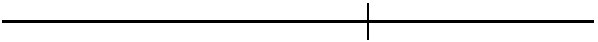
\includegraphics[width=0.7\textwidth]{golden-ratio}
  \end{center}

  \begin{theorem}Der goldene Schnitt~$\Phi$ ist die \hil{irrationalste aller
  Zahlen}.\end{theorem}
  \medskip
  \textbf{Beweis.} $\Phi = \icfrac{1}{1}{1}{1}.$
\end{frame}

\note{\justifying
  The golden ratio appears in lots of places in nature and art. If you divide a
  segment in the golden ratio, the longer subsegment will be~$\Phi$ times as
  long as the shorter subsegment; more conceptually:
  \[ \footnotesize \text{total segment} : \text{longer subsegment} =
    \text{longer subsegment} : \text{shorter subsegment}. \]

  If you use a fraction~$\frac{a}{b}$ of the full circle as rotation angle,
  then after~$b$ turns you'll arrive at exactly the same location as you
  started. That's bad! Space is wasted this way.
  \medskip

  It's better to use a number which can \emph{not} be expressed as a fraction
  -- an \emph{irrational number}. Of all irrational numbers, one should pick
  the \emph{most irrational} one.
  \medskip

  Recall that a number can the better be approximated by fractions the larger
  the coefficients in the continued fraction expansion are. With~$\Phi$, the
  coefficients are as small as possible. This is the reason why~$\Phi$ is the
  ``most irrational'' number. It is the hardest number to approximate by
  fractions.\par
}

\begin{frame}\frametitle{(Nicht-)Verwendung des goldenen Winkels}
  \centering
  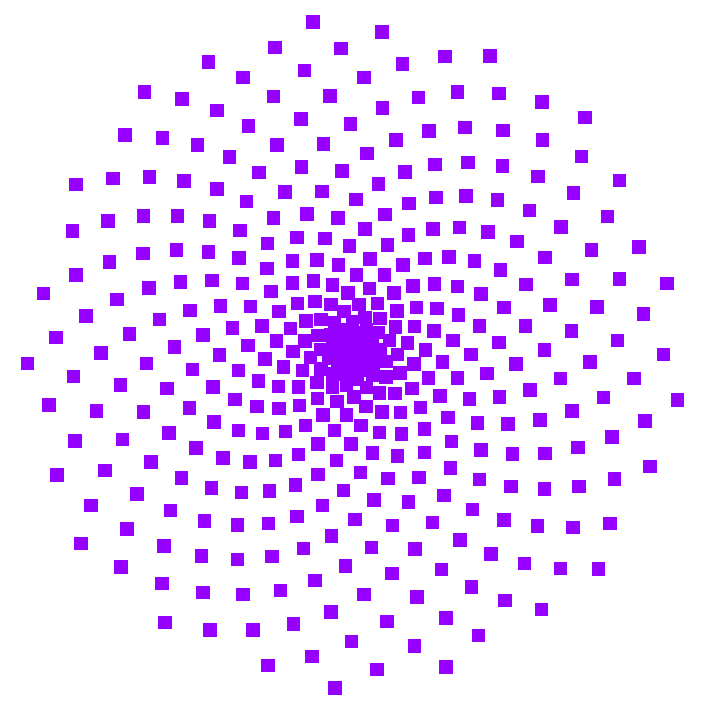
\includegraphics[width=0.45\textwidth]{drehwinkel-400-1_61803398874989484820.pdf}

  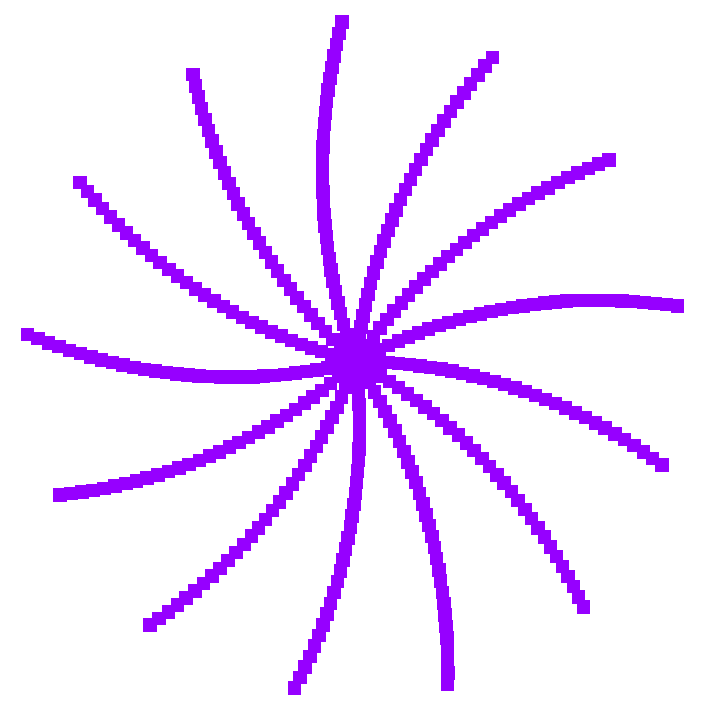
\includegraphics[width=0.25\textwidth]{drehwinkel-400-1_61525621097211707043.pdf}
  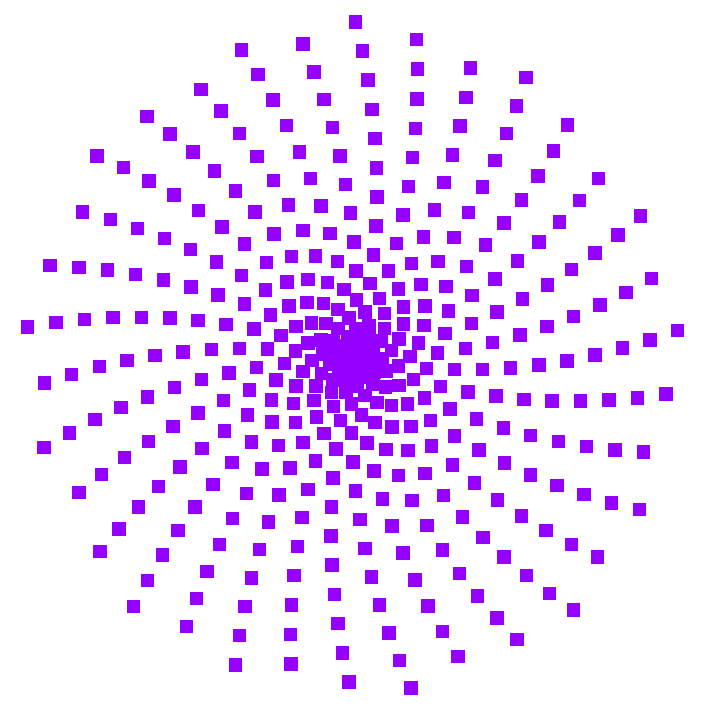
\includegraphics[width=0.25\textwidth]{drehwinkel-400-1_61775621097211707043.pdf}
  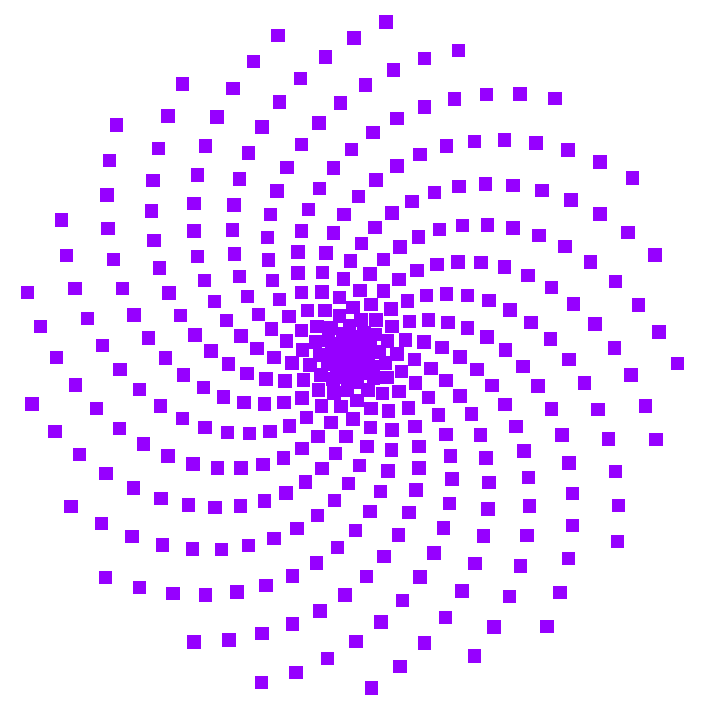
\includegraphics[width=0.25\textwidth]{drehwinkel-400-1_61831176652767262597.pdf}
  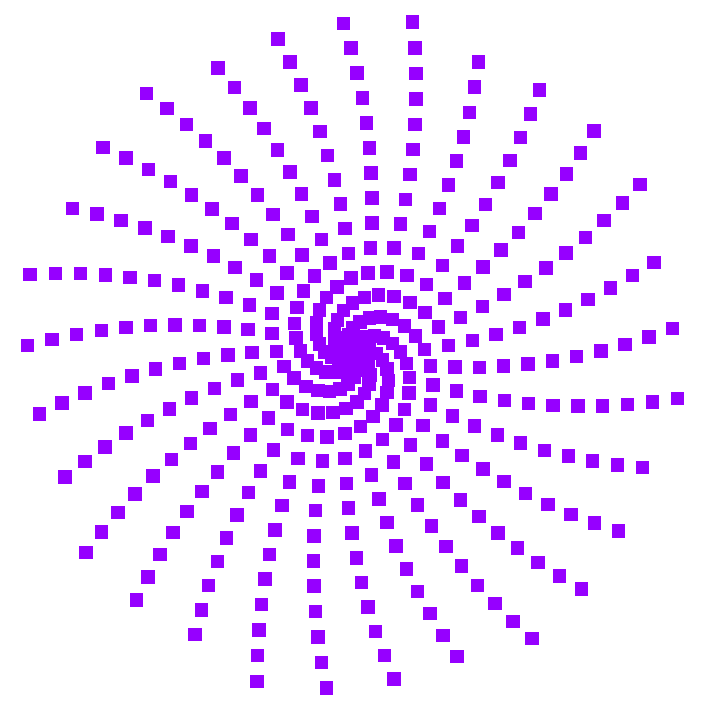
\includegraphics[width=0.25\textwidth]{drehwinkel-400-1_62081176652767262597.pdf}
  \par
\end{frame}

\note{\justifying
  The top figure uses the golden angle. The angles used in the four
  figures in the bottom are:
  \begin{enumerate}
    \item $\text{golden angle} - 1^\circ$
    \item $\text{golden angle} - 0.1^\circ$
    \item $\text{golden angle} + 0.1^\circ$
    \item $\text{golden angle} + 1^\circ$
  \end{enumerate}

  You are invited to write a fancy interactive JavaScript/canvas demo. Use the
  following simple formulas for the coordinates of the~$n$'th point,
  where~$\varphi$ is the given angle to use ($\varphi = 1/4$ meaning 90
  degrees).
  \begin{align*}
    x &= n \cdot \cos(2 \pi \varphi \cdot n) \\
    y &= n \cdot \sin(2 \pi \varphi \cdot n)
  \end{align*}
}

\note{\centering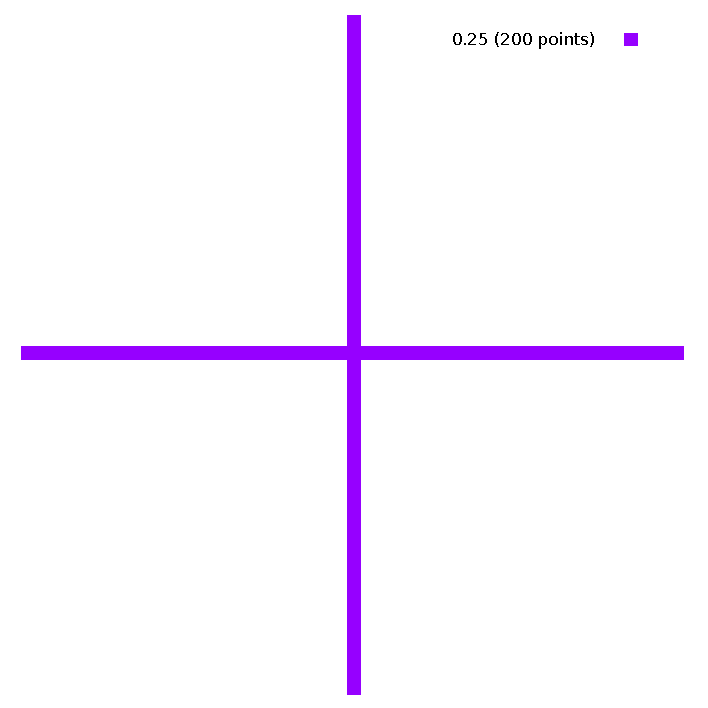
\includegraphics[height=0.95\textheight]{drehwinkel-200-0_25.pdf}\par}
\note{\centering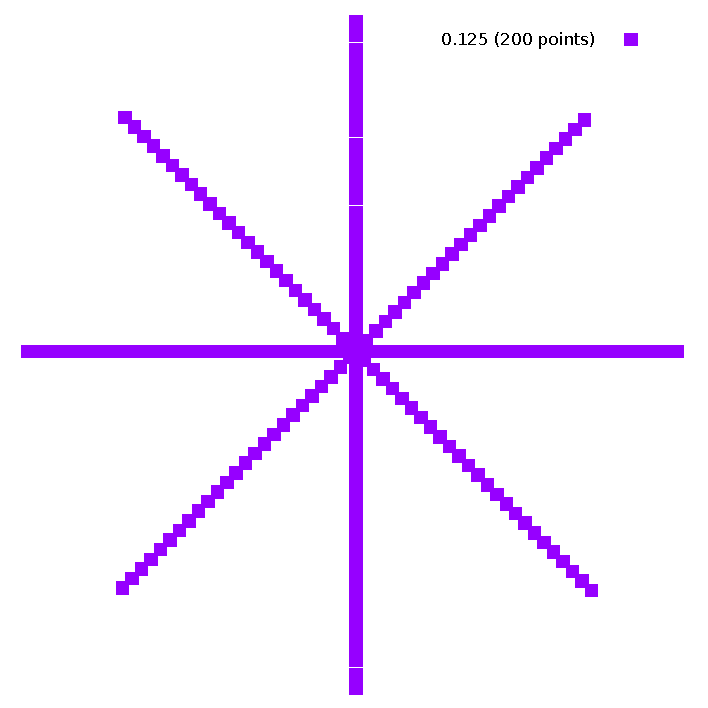
\includegraphics[height=0.95\textheight]{drehwinkel-200-0_125.pdf}\par}
\note{\centering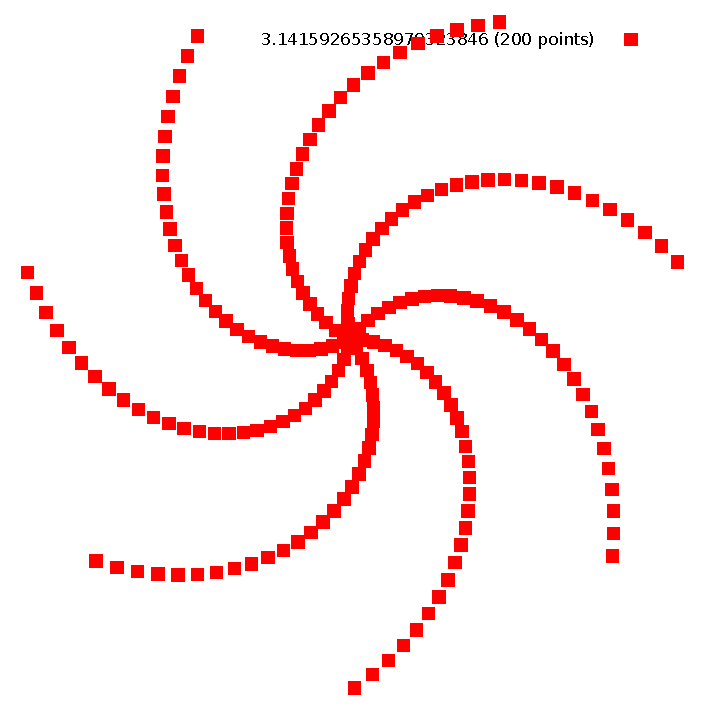
\includegraphics[height=0.95\textheight]{drehwinkel-200-3_14159265358979323846.pdf}\par}
\note{\centering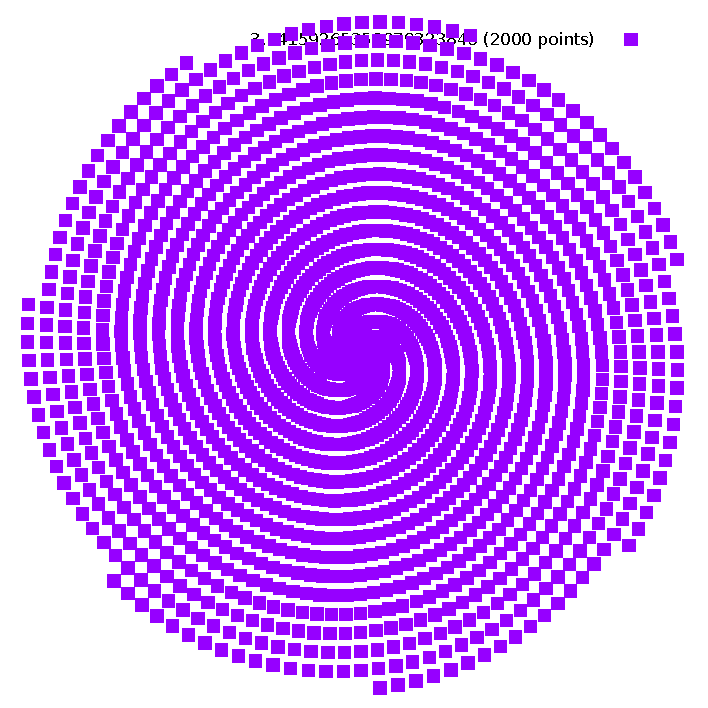
\includegraphics[height=0.95\textheight]{drehwinkel-2000-3_14159265358979323846.pdf}\par}
\note{\centering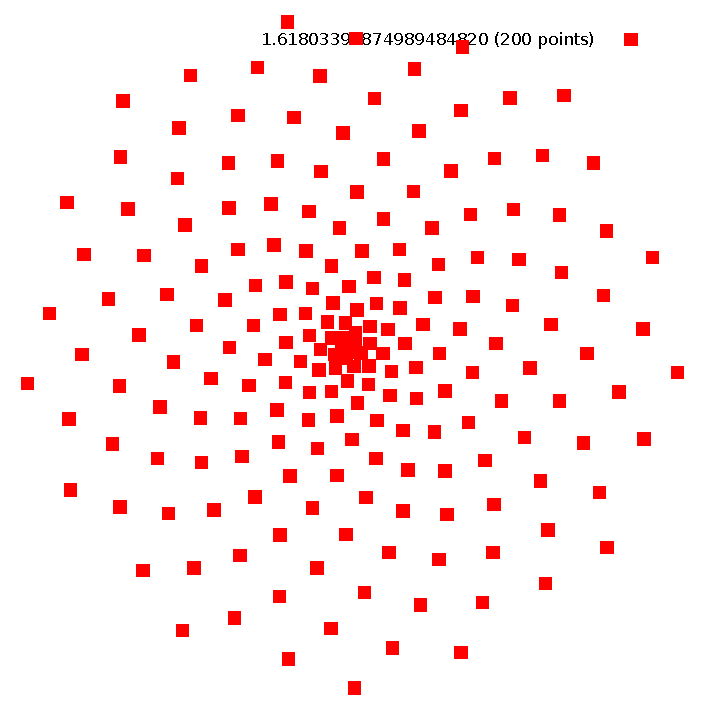
\includegraphics[height=0.95\textheight]{drehwinkel-200-1_61803398874989484820.pdf}\par}
\note{\centering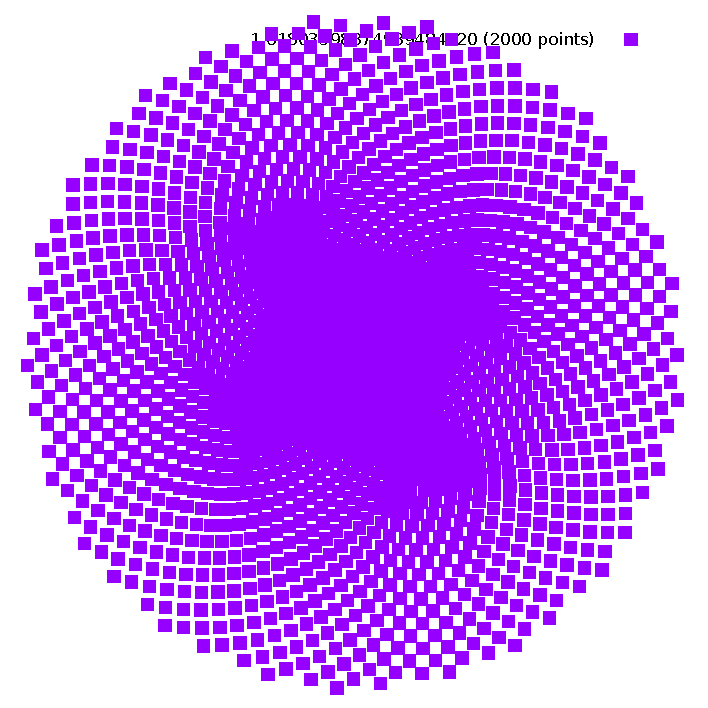
\includegraphics[height=0.95\textheight]{drehwinkel-2000-1_61803398874989484820.pdf}\par}

\begin{frame}\frametitle{Wieso die Fibonaccizahlen?}
  \vspace*{-1em}
  \[ \Phi = \icfrac{1}{1}{1}{1} \]

  \begin{enumerate}
    \item $1\phantom{[,1,1,1,1,1,1,1,1]} = \phantom{0}1/1$
    \item $[1;1]\phantom{,1,1,1,1,1,1,1} = \phantom{0}2/1$
    \item $[1;1,1]\phantom{,1,1,1,1,1,1} \pause = \phantom{0}3/2$
    \item $[1;1,1,1]\phantom{,1,1,1,1,1} \pause = \phantom{0}5/3$
    \item $[1;1,1,1,1]\phantom{,1,1,1,1} \pause = \phantom{0}8/5$ \pause
    \item $[1;1,1,1,1,1]\phantom{,1,1,1} = 13/8$
    \item $[1;1,1,1,1,1,1]\phantom{,1,1} = 21/13$
    \item $[1;1,1,1,1,1,1,1]\phantom{,1} = 34/21$
    \item $[1;1,1,1,1,1,1,1,1] = 55/34$
  \end{enumerate}
\end{frame}

\note{\justifying
  Using a fraction~$\frac{a}{b}$ of the full circle as rotation angle (given in
  lowest terms) yields precisely~$b$ spirals. The animation at
  \[ \text{\scriptsize\url{http://rawgit.com/iblech/number5/master/drehwinkel-0_3027522935779816.mp4}} \]
  shows a zoom when using~$33/109$ as rotation angle. Its
  continued fraction expansion is
  \[ \frac{33}{109} = \dfrac{1}{3 + \dfrac{1}{3 + \dfrac{1}{3 +
  \dfrac{1}{3}}}} \]
  with truncations
  \[ \dfrac{1}{3}, \qquad
  \dfrac{1}{3 + \dfrac{1}{3}} = \dfrac{3}{10}, \qquad
  \dfrac{1}{3 + \dfrac{1}{3 + \dfrac{1}{3}}} = \dfrac{10}{33}.
  \]
  Therefore you first see three, then ten, then 33, and finally 109 spirals.
}


\section{Die Ananas aus SpongeBob Schwammkopf}

\begin{frame}\frametitle{Die Ananas aus SpongeBob Schwammkopf}
  \centering
  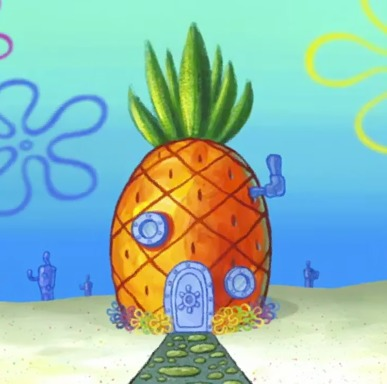
\includegraphics[width=0.65\textwidth]{spongebob-ananas}
  \medskip

  Von Vi Hart, Mathemusikerin.
  \par
\end{frame}

\note{\justifying
  Watch
  \emph{Open Letter to Nickelodeon, Re: SpongeBob's Pineapple under the Sea} by
  Vi Hart on YouTube: \url{https://www.youtube.com/watch?v=gBxeju8dMho}\par

  \centering
  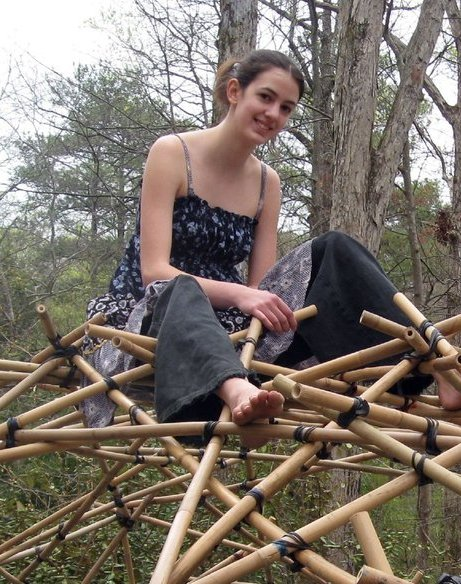
\includegraphics[width=0.3\textwidth]{vi-hart}
  \bigskip

  \emph{Check out an exercise sheet for more fun:} \\[0.2em]
  \scriptsize
  \url{http://rawgit.com/iblech/number5/master/pizzaseminar-en.pdf}
  \url{http://rawgit.com/iblech/number5/master/pizzaseminar-de.pdf}%
  \\
  Exercise 12 explains the relation between the golden ratio and the number~5.
  \bigskip

  \scalebox{2.8}{\large\hil{$\boldsymbol{\heartsuit}$}}
  \par
}

\appendix

\backupstart

\section{Bildquellen}

\begin{frame}\frametitle{Image sources}
  \tiny
  \url{https://upload.wikimedia.org/wikipedia/commons/9/99/Vi_Hart.jpg}
  \url{http://joachim-reichel.org/software/fraktal/mandelbrot_large.png}
  \url{https://commons.wikimedia.org/wiki/File:Bellis_perennis_white_(aka).jpg}
  \url{http://www.maths.surrey.ac.uk/hosted-sites/R.Knott/Fibonacci/coneflower.jpg} (Tim Stone)
  \url{http://www.bibliotecapleyades.net/imagenes_ciencia2/conscious_universe472_02.jpg}
  \url{http://www.education.txstate.edu/ci/faculty/dickinson/PBI/PBIFall06/GeoNature/Content/Fibonacci_Lesson_files/image037.gif}
  \mbox{\url{http://www.sciencedump.com/sites/default/files/styles/article_width/public/field/gallery/8247962.jpg}}
  \par
\end{frame}

\backupend

\end{document}

Plan of the talk:

1. Images of spirals in nature; notice Fibonacci numbers.
2. Infinite continued fraction:
   * Example with [1; 2, ...]
   * More examples (only listed)
   * Euclidean algorithm (with illustration?)
   * Theorem about best approximation
3. Approximation of pi
   * List original sources for 22/7 and 355/113
   * Explain using continued fractions
4. Spirals in nature
   * angle, need "most irrational number"
   * golden ratio (also explain as a ratio)
   * simulations
5. Fibonacci numbers in the Mandelbrot fractal
6. Vi Hart

Mention rational tangles?

Relation to the number 5.
